\documentclass[10pt, a4paper, twocolumn]{article}

\usepackage{amsmath, amsthm, amssymb}
\usepackage[top=0.7in, bottom=0.75in, left=0.65in, right=0.65in, columnsep=0.25in]{geometry}
\usepackage{graphicx}
\usepackage{booktabs}
\usepackage{caption}
\usepackage[bidi=bidi]{babel}
\babelprovide[import, main]{hebrew}
\babelprovide[import]{english}
\usepackage{fontspec}
\babelfont{rm}{Times New Roman}
\babelfont{sf}{Arial}
\babelfont{tt}{Courier New}

\captionsetup{font=footnotesize, labelfont=bf, skip=3pt}

\newtheorem{theorem}{משפט}
\newtheorem{proposition}{טענה}
\newtheorem{assumption}{הנחה}
\newtheorem{remark}{הערה}

\title{\vspace{-1.2em}\Large\textbf{ניווט \foreignlanguage{english}{I-Bug} חסין תחת מתקפת התחזות אותות לסירוגין}\\
\normalsize\foreignlanguage{english}{\textbf{Resilient I-Bug Navigation under Intermittent Signal Spoofing}}}

\author{
  \textbf{צוריאל ויזל} \quad \textbf{אברהם גז} \\
  \small מנחה: ד"ר אנדריי ז'יטניקוב \\
  \small הטכניון -- מכון טכנולוגי לישראל \\
  \vspace{-1.2em}
}
\date{}

\begin{document}

\maketitle

\begin{abstract}
\noindent
רובוטים אוטונומיים מינימליסטיים הפועלים בסביבות חסומות \foreignlanguage{english}{GPS} מסתמכים על משוב חיישנים מקומי במקום על קואורדינטות גלובליות או אודומטריה. אלגוריתם ה-\foreignlanguage{english}{I-Bug} משיג התכנסות מובטחת למטרה באמצעות חיישן מגע וחיישן עוצמת אות סקלרי בלבד. עם זאת, במערכות חישה לא-קוהרנטיות שבהן המקלט מודד סכום חיבורי של תרומות ממספר משדרים, ניווט מבוסס-עוצמה חשוף באופן חמור למתקפות התחזות (\foreignlanguage{english}{Spoofing}) לסירוגין. משדר תוקף חיבורי מעוות את גרדיאנט העוצמה המרחבי במרחב החופשי ומזריק נקודות מקסימום כוזבות לאורך שפות מכשולים, ובכך לוכד סוכני \foreignlanguage{english}{I-Bug} סטנדרטיים בלולאות אינסופיות. במאמר זה אנו מציגים מסנן אנומליות זמני מבוסס-קינמטיקה ושתי אסטרטגיות נגד — אסטרטגיה \textit{זהירה} (\foreignlanguage{english}{Cautious}) המשמרת באופן מותנה את הבטחת ההתכנסות של \foreignlanguage{english}{I-Bug} התקין תחת מודל האיום שלנו, והיוריסטיקה \textit{אינרציאלית} (\foreignlanguage{english}{Inertial}) מהירה בחוג פתוח — ללא צורך בשום חומרה נוספת. באמצעות ניצול הפרדת סדרי הגודל בין שינויי עוצמה מרחביים החסומים קינמטית לבין אי-רציפויות מיתוג של התוקף בזמן, המסנן שלנו מבודד פרצי תקיפה בזמן אמת. אנו מוכיחים משפט שימור מותנה המראה כי תחת התחזות מדרגה לסירוגין (הנחות 1–2), האסטרטגיה הזהירה משמרת את מסלול המצבים הפעילים המדויק של כל ריצת \foreignlanguage{english}{I-Bug} תקינה מתכנסת, ומוכיחים כי הקפאת זיכרון בלבד תוך המשך תנועת שפה דטרמיניסטית אינה מספיקה להתכנסות אוניברסלית עקב נעילת פאזה טופולוגית (תהודה / \foreignlanguage{english}{Resonance}). הערכות מזווגות על פני $1,000,000$ סביבות מכשולים דו-ממדיות אקראיות מראות כי תחת התפלגות הסביבות שנדגמה, אלגוריתם הבסיס התמים (\foreignlanguage{english}{Naive I-Bug}) מצליח ב-$54.68\% \pm 0.10\%$ בלבד מההרצות, ההיוריסטיקה האינרציאלית משיגה $99.61\% \pm 0.01\%$ הצלחה תוך קיצור ממוצע הצעדים בריצות מוצלחות ב-$20.5\%$, והאסטרטגיה הזהירה משיגה $100.00\%$ הצלחה נצפית (רווח בר-סמך \foreignlanguage{english}{Clopper--Pearson} של $95\%$: $[99.9996\%, 100.00\%]$).
\end{abstract}

\section{מבוא ומודל האיום}
ניווט \foreignlanguage{english}{Bug} קלאסי מספק הבטחות התכנסות בסביבות מישוריות לא ידועות באמצעות חישה מקומית מוגבלת \cite{lumelsky1987path, kamon1998tangentbug}, בעוד שאלגוריתם ה-\foreignlanguage{english}{I-Bug} מחליף מידע קואורדינטות וטווח בעוצמת האות ממשדר המטרה \cite{taylor2009ibug, taylor2014intensity}. בגבול תאורטי זה של מינימליזם חישתי, רובוט דמוי-דיסקה ברדיוס $r_c > 0$ מנווט במרחב עבודה מישורי חסום $\mathcal{W} \subset \mathbb{R}^2$ המכיל אוסף סופי של מכשולים לא ידועים $\mathcal{O} = \{O_1, \dots, O_M\}$ (עם מרחב תצורה חופשי מהתנגשות $\mathcal{F} \subset \mathcal{W}$) באמצעות פגוש מגע מקומי וחיישן סקלרי המודד עוצמת שידור ממגדל מטרה לא ידוע $p_t \in \mathcal{F}$.

בתנאים תקינים, עוצמת המטרה היא פונקציה רדיאלית יורדת ממש של המרחק האוקלידי, $m(p - p_t) = \|p - p_t\|_2^{-1}$, והמשימה מסתיימת בהצלחה כאשר $\|p - p_t\|_2 < R_{\text{reach}}$. ללא קואורדינטות או אודומטריה, הרובוט מבצע שלוש פעולות בסיסיות בצעדי בקרה בדידים $k \in \mathbb{N}_0$ (זמן צעד $\Delta t$, גודל צעד $\Delta s = v_{\max}\Delta t$):
\begin{enumerate}
    \item $u_{\text{ori}}$ (\textbf{כיוון לגרדיאנט}): מיישר את זווית הכיוון $\theta_k$ עם שערוך כיוון גרדיאנט מקומי המתקבל מדגימות מרחביות קרובות של אותו חיישן עוצמה סקלרי $S(p, t)$:
    \begin{equation}
        \theta_{\nabla}(p, t) = \operatorname{atan2}\!\bigl(\partial_y S(p, t),\, \partial_x S(p, t)\bigr) \pmod{2\pi}.
        \label{eq:grad_angle}
    \end{equation}
    \item $u_{\text{fwd}}$ (\textbf{תנועה קדימה}): צועד ליניארית בכיוון $\theta_k$ במצב מרחב חופשי \foreignlanguage{english}{\texttt{MoveToTower}}. בעת מגע עם מכשול, הרובוט מתעד את סף הפגיעה $i_H \leftarrow \max(S(p_k, t_k), i_H)$, פונה ימינה ב-$\pi/2$, ועובר למצב \foreignlanguage{english}{\texttt{FollowObstacle}}.
    \item $u_{\text{fol}}$ (\textbf{מעקב שפה}): עוקב אחר היקף המכשול תוך שמירת הקיר משמאלו ועדכון המקסימום המקומי $i_{\text{max}}$. ברגע שהרובוט טיפס מעל הסף ($i_{\text{max}} > i_H + \epsilon$) וזיהה לאחריו דגימה יורדת ($S(p_k, t_k) < i_{\text{max}} - \epsilon$), הוא מעדכן $i_H \leftarrow i_{\text{max}}$, מפעיל $u_{\text{ori}}$ וחוזר ל-\foreignlanguage{english}{\texttt{MoveToTower}}.
\end{enumerate}

\noindent\textbf{מודל סופרפוזיציית \foreignlanguage{english}{RSS} חיבורי עוין.}
אותות ניווט מזויפים יכולים לתמרן פלטפורמות אוטונומיות, בעוד שתוקפים מתוחכמים עשויים להפעיל השתלטות אות לסירוגין או באופן סמוי כדי לשבש את ההנחיה \cite{kerns2014unmanned, psiaki2016gnss}. נבחן משדר תוקף במיקום לא ידוע $p_e \in \mathcal{F}$ המשדר אות התחזות לסירוגין בעוצמה $\alpha_e > 0$ הנשלטת על ידי פונקציית מיתוג $u(t) \in \{0, 1\}$.

\begin{assumption}[שדה סופרפוזיציית \foreignlanguage{english}{RSS} חיבורי]
\label{assump:superposition}
אנו חוקרים הפשטה של עוצמת אות נקלט (\foreignlanguage{english}{RSS}) חיבורית לא-קוהרנטית שבה החיישן מדווח את סכום תרומות המקור הלגיטימי והתוקף במיקום $p \in \mathcal{F}$ ובזמן $t \ge 0$:
\begin{equation}
    S(p, t) = m(p - p_t) + e(p, t), \quad e(p, t) = u(t)\,\frac{\alpha_e}{\|p - p_e\|_2}.
    \label{eq:superposition}
\end{equation}
\end{assumption}

כאשר $u(t) = 1$, הרכיב העוין $e(p, t)$ משחית הן את הקריאה הסקלרית $S(p, t)$ והן את הגרדיאנט המרחבי שלה:
\begin{equation}
    \nabla_p S(p, t) = -\frac{p - p_t}{\|p - p_t\|_2^3} - u(t)\,\alpha_e \frac{p - p_e}{\|p - p_e\|_2^3}.
    \label{eq:corrupted_grad}
\end{equation}
כתוצאה מכך, רובוט לא מוגן מוסת ממסלולו במהלך $u_{\text{ori}}$ ומתעד ספי פגיעה מורעלים $i_H$ בעת מגע עם מכשול שאינם ניתנים למעבר לאחר ש-$u(t) \to 0$, מה שלוכד את הרובוט בלולאות מעקב-שפה אינסופיות.

\section{גילוי אנומליות מבוסס-פיזיקה ואסטרטגיות נגד}

בהשראת גילוי מתקפות מבוסס-פיזיקה \cite{giraldo2018survey} וגילוי שינויים חדים קלאסי \cite{basseville1993detection}, אנו מגנים על הרובוט ללא חומרה נוספת או גישת אורקל ל-$m(p - p_t)$ על ידי ניצול ההפרדה בין שינוי עוצמה חסום הנובע מתנועה לבין מיתוג משדר אי-רציף.

\begin{assumption}[חסם ליפשיץ קינמטי לעומת אי-רציפות זמנית]
\label{assump:discontinuity}
על פני חלון דגימת חיישן בקצב גבוה $\delta t \ll \Delta t$ (העתקה מרחבית מקסימלית $\delta s = v_{\max}\delta t \ll R_{\text{reach}}$) שבמהלכו התוקף כבוי ($u \equiv 0$), שינוי העוצמה הטבעי מעוצמת ייחוס $I_{\text{ref}} = m(p - p_t) = 1/d$ חסום על ידי תוספת ליפשיץ הרדיאלית המקומית:
\begin{equation}
    \Delta I_{\max}(I_{\text{ref}}) = \frac{\delta s}{d(d - \delta s)} = \frac{\delta s\, I_{\text{ref}}^2}{1 - \delta s\, I_{\text{ref}}}.
    \label{eq:lipschitz}
\end{equation}
מנגד, $u(t)$ ממתג בין $0$ ל-$1$ עם משך פעילות $T_{\text{on}} \ge 1$ צעדים ומשך השבתה $T_{\text{off}} > N_{\text{confirm}}$ צעדים, ומייצר קפיצת מדרגה מיידית
\begin{equation}
    e_{\min} := \frac{\alpha_e}{\max_{p \in \mathcal{F}_{\text{nav}}} \|p - p_e\|_2} \ge \frac{\alpha_e}{\operatorname{diam}(\mathcal{W})}
    \label{eq:emin_short}
\end{equation}
המקיימת $e_{\min} > \eta_{\text{spike}} \max_{p \in \mathcal{F}_{\text{nav}}} \Delta I_{\max}(m(p-p_t))$.
\end{assumption}

\begin{remark}[מוטיבציה פיזיקלית, תחום חלות ורעש חסום]
הנחה~\ref{assump:discontinuity} מבוססת על הפרדת סדרי גודל בזמן: דגימה אלקטרונית ($\text{kHz}$) מהירה בסדרי גודל מתנועה מכנית ($v_{\max}$), ולכן $\delta s = v_{\max}\delta t$ ו-$\Delta I_{\max}$ קטנים מאוד ביחס לקפיצות מיתוג. ההבטחה התאורטית אינה חלה על מתקפות הפועלות ברציפות, מתקפות בעלות שיפוע איטי (\foreignlanguage{english}{Slowly Ramped}), או מתקפות מתחת לסף הגילוי שבהן השארית הזמנית נותרת מתחת לסף \cite{psiaki2016gnss}; ניתוח פורמלי של מתקפות חמקניות כאלה מושאר לעבודה עתידית. תחת רעש מדידה חסום $|\nu_k| \le \varepsilon_{\text{noise}}$, התראות שווא נמנעות אם $\Delta I_{\max} + 2\varepsilon_{\text{noise}} < \eta_{\text{spike}}\Delta I_{\max}$, והחמצות גילוי נמנעות אם $e_{\min} - 2\varepsilon_{\text{noise}} > \eta_{\text{spike}}\Delta I_{\max}$ (ובאופן אנלוגי עבור $\mathcal{A}_{\text{drop}}$ עם $\eta_{\text{drop}} \le \eta_{\text{spike}}$).
\end{remark}

\noindent\textbf{מסנן האנומליות.}
בתחילת צעד $k$ (לפני תנועה), המסנן משווה את קריאת תחילת הצעד $I_k^- = S(p_{k-1}, t_k)$ מול קריאת סוף הצעד הקודם $I_{k-1}^+ = S(p_{k-1}, t_{k-1})$. נשים לב כי במעבר הדלקה ($0 \to 1$), הקריאה $I_{k-1}^+ = m(p_{k-1}-p_t)$ נקייה משיבוש, ואילו במעבר כיבוי ($1 \to 0$), הקריאה $I_k^- = m(p_{k-1}-p_t)$ נקייה משיבוש. עם $\Delta I_k = I_k^- - I_{k-1}^+$, אנומליות חיוביות (\foreignlanguage{english}{\textit{spike}}) ושליליות (\foreignlanguage{english}{\textit{drop}}) מזוהות לפי:
\begin{align}
    \mathcal{A}_{\text{spike}} &\iff \Delta I_k > \eta_{\text{spike}}\,\Delta I_{\max}(I_{k-1}^+), \label{eq:spike} \\
    \mathcal{A}_{\text{drop}} &\iff (-\Delta I_k > 0.15 I_{k-1}^+) \;\lor \nonumber\\
    &\qquad\quad (-\Delta I_k > \eta_{\text{drop}}\Delta I_{\max}(I_k^-)), \label{eq:drop}
\end{align}
כאשר $\eta_{\text{spike}} = 2.0$ ו-$\eta_{\text{drop}} = 1.2$. אנו בוחנים שלוש אסטרטגיות:
\begin{itemize}
    \item \textbf{תמימה (\foreignlanguage{english}{Naive} -- בסיס \foreignlanguage{english}{I-Bug} המקורי \cite{taylor2014intensity}):} עוקפת את המסנן, ומבצעת $u_{\text{ori}}, u_{\text{fwd}}, u_{\text{fol}}$ ועדכוני $i_H$ ישירות על $S(p, t)$.
    \item \textbf{זהירה (\foreignlanguage{english}{Cautious} -- הקפאת מצב):} עם זיהוי $\mathcal{A}_{\text{spike}}$, הרובוט עובר למצב \foreignlanguage{english}{\texttt{Paused}}: הוא עוצר במקום ($\Delta p_k = 0$), נועל את תנוחתו $(p_{\text{frozen}}, \theta_{\text{frozen}})$ ואת זיכרונו הפנימי $(i_H, i_{\text{max}}, i_{\text{mem}})$, וממתין עד לזיהוי $\mathcal{A}_{\text{drop}}$ ואימות של $N_{\text{confirm}} = 3$ צעדים יציבים רצופים לפני חזרה לניווט \foreignlanguage{english}{\texttt{Normal}}.
    \item \textbf{אינרציאלית (\foreignlanguage{english}{Inertial} -- היוריסטיקת חוג פתוח):} עם זיהוי $\mathcal{A}_{\text{spike}}$, הרובוט עובר ל-\foreignlanguage{english}{\texttt{InertialMode}}: הוא מקפיא את כיוונו $\theta_{\text{frozen}}$ ומשהה עדכוני זיכרון ושיאים, אך ממשיך לנוע. ב-\foreignlanguage{english}{\texttt{MoveToTower}}, הוא מדכא את $u_{\text{ori}}$ וצועד ישר דרך $u_{\text{fwd}}$ (ומאתחל $i_H \leftarrow i_{\text{mem}}$ מזיכרונו הנקי האחרון אם פגע במכשול). ב-\foreignlanguage{english}{\texttt{FollowObstacle}}, הוא ממשיך במעקב שפה פיזי דרך $u_{\text{fol}}$ תוך השהיית תנאי העזיבה עד ש-$\mathcal{A}_{\text{drop}}$ מחזיר אותו למצב \foreignlanguage{english}{\texttt{Normal}}.
\end{itemize}

\section{ניתוח התכנסות פורמלי ותהודה}

\begin{theorem}[שימור מותנה של מסלול המצבים הפעילים וההתכנסות]
\label{thm:cautious}
תחת הנחות~\ref{assump:superposition} ו-\ref{assump:discontinuity} עם $\eta_{\text{drop}} \le \eta_{\text{spike}}$ ו-$T_{\text{off}} > N_{\text{confirm}}$, עבור כל מרחב עבודה $\mathcal{W}$ ושדה תקין $m$:
(א) עקבת המיקומים המרחביים $\gamma_{\text{cautious}}$ והמצבים הפנימיים בצעדים הפעילים זהים לחלוטין לריצת ה-\foreignlanguage{english}{I-Bug} התקינה $\gamma_{\text{ideal}}$; ו-(ב) בכל סביבה שבה הריצה התקינה מגיעה ל-$\|p_k - p_t\|_2 < R_{\text{reach}}$ תוך $N_{\text{ideal}} < \infty$ צעדים פעילים (ובפרט תחת הנחות ההתכנסות של \cite{taylor2014intensity}), הרובוט הזהיר מגיע למטרה תוך לכל היותר
\begin{equation}
    N_{\text{cautious}} \le N_{\text{ideal}} + \left\lceil \frac{N_{\text{ideal}}}{T_{\text{off}} - N_{\text{confirm}}} \right\rceil (T_{\text{on}} + N_{\text{confirm}})
    \label{eq:bound}
\end{equation}
צעדים סופיים.
\end{theorem}

\begin{proof}
בכל צעד הפעלת תוקף $k_j^{\text{on}}$, מתקיים $\Delta I_k = m_e(p_{k-1} - p_e) \ge e_{\min} > \eta_{\text{spike}}\Delta I_{\max}(I_{k-1}^+)$, מה שמפעיל את $\mathcal{A}_{\text{spike}}$ לפני תנועה או שינוי זיכרון. לאורך $[k_j^{\text{on}}, k_j^{\text{off}}-1]$, המיקום $p_k$ נייח והמצב המלא $\Sigma_k = (p_k, \theta_k, \text{mode}, i_H, i_{\text{max}}, i_{\text{mem}})$ נעול. בצעד הכיבוי $k_j^{\text{off}}$, מאחר ש-$\eta_{\text{drop}} \le \eta_{\text{spike}}$, הנפילה $-m_e(p_{k-1}-p_e) \ge e_{\min} > \eta_{\text{drop}}\Delta I_{\max}(I_{k_j^{\text{off}}}^-)$ מפעילה את $\mathcal{A}_{\text{drop}}$, ולאחר $N_{\text{confirm}}$ צעדי אימות נייחים שבהם $u(t)=0$, הרובוט חוזר לפעולה ב-$k_j^{\text{res}} = k_j^{\text{off}} + N_{\text{confirm}} - 1$ עם $\Sigma(k_j^{\text{res}}) = \Sigma(k_j^{\text{on}} - 1)$. לכן, בכל צעד פעיל $\tau$, $u(t_k) = 0 \implies S(p, t_k) = m(p - p_t)$ ו-$\nabla_p S = \nabla_p m$. באינדוקציה על הצעדים הפעילים $\tau$, $\Sigma(\tau) \equiv \Sigma_{\text{ideal}}(\tau)$, ולכן $\gamma_{\text{cautious}} \equiv \gamma_{\text{ideal}}$. כאשר $\gamma_{\text{ideal}}$ מתכנס ב-$N_{\text{ideal}} < \infty$ צעדים, כל מחזור מספק $T_{\text{off}} - N_{\text{confirm}} \ge 1$ צעדים פעילים עבור $T_{\text{on}} + N_{\text{confirm}}$ צעדים מושהים, ומכאן משוואה~\eqref{eq:bound}.
\end{proof}

\begin{proposition}[אי-מספיקות של הקפאת זיכרון בלבד]
\label{prop:resonance}
הקפאת זיכרון פנימי בלבד תוך המשך תנועת שפה דטרמיניסטית אינה מספיקה להבטחת התכנסות אוניברסלית. תהא $\mathcal{A}_L \subset \partial O_i$ קשת זיהוי היציאה על שפת מכשול $O_i$ בעל היקף $L_i$, שעל פניה יש להשלים את סדרת היציאה (טיפוס מעל $i_H + \epsilon$, שיא $i_{\max}$, וירידה ב-$\epsilon$). אם זמן ההקפה $T_{\text{orbit}} = L_i / (v_{\text{fol}}\Delta t)$ מקיים סנכרון פאזה $T_{\text{orbit}} = m\,T_{\text{cycle}}$ ($m \in \mathbb{N}$) והקשת העיוורת באורך $v_{\text{fol}} T_{\text{on}}\Delta t$ במהלך $[k_j^{\text{on}}, k_j^{\text{off}})$ מכסה את $\mathcal{A}_L$, הרובוט האינרציאלי יחלוף על פני $\mathcal{A}_L$ בזמן שזיהוי השיא מושהה בכל הקפה עוקבת, ויילכד בלולאת גבול אינסופית (בעוד שמחזורים קרובים $T_{\text{orbit}} \approx m\,T_{\text{cycle}}$ גורמים ללכידה ממושכת אך סופית).
\end{proposition}

\section{הערכה אמפירית בקנה מידה רחב}
מימשנו סימולטור קינמטי דו-ממדי רציף בשפת \foreignlanguage{english}{Julia} ($\mathcal{W} = [0, 20]^2$, $p_0 = (2, 1)$, $p_t = (18, 18)$, $R_{\text{reach}} = 0.5$, $r_c = \Delta s = 0.3$, $T_{\text{cycle}} = 40$, $T_{\text{on}} = 10$, $\alpha_e = 1.0$, אופק $N_{\max} = 2,000$). על פני $1,000,000$ מבוכים מוגרלים (10–16 קירות מלבניים חופפים עם מעברים רחבים ושוליים היקפיים), שלוש האסטרטגיות הוערכו בניסויים מזווגים.

\begin{table}[htbp]
\centering
\scriptsize
\setlength{\tabcolsep}{2.2pt}
\vspace{-0.4em}
\caption{הערכה מזווגת ($10^6$ הרצות; מדדי צעדים בריצות מוצלחות לעומת כלל ההרצות עם קנס אופק)}
\label{tab:results}
\resizebox{\linewidth}{!}{%
\begin{tabular}{@{}lcccc@{}}
\toprule
\textbf{אסטרטגיה} & \textbf{הצלחה (\foreignlanguage{english}{$95\%$ CI})} & \textbf{ממוצע (מוצלחות)} & \textbf{חציון [\foreignlanguage{english}{IQR}] (מוצלחות)} & \textbf{$\bar{N}_{\text{capped}}$} \\ \midrule
\foreignlanguage{english}{Naive} \cite{taylor2014intensity} & \foreignlanguage{english}{$54.68\% \pm 0.10\%$}  & \foreignlanguage{english}{$199.3$} & \foreignlanguage{english}{$153.0$ $[121,\, 205]$} & \foreignlanguage{english}{$1015.4$} \\
\foreignlanguage{english}{Cautious} & \foreignlanguage{english}{$\mathbf{100.00\%}$ ($[99.9996, 100]$)} & \foreignlanguage{english}{$193.0$} & \foreignlanguage{english}{$178.0$ $[160,\, 215]$} & \foreignlanguage{english}{$193.0$} \\
\foreignlanguage{english}{Inertial} & \foreignlanguage{english}{$99.61\% \pm 0.01\%$}  & \foreignlanguage{english}{$\mathbf{153.4}$} & \foreignlanguage{english}{$\mathbf{135.0}$ $[115,\, 168]$} & \foreignlanguage{english}{$\mathbf{160.6}$} \\ \bottomrule
\end{tabular}%
}
\vspace{-1.2em}
\end{table}

\begin{figure}[htbp]
    \centering
    \begin{minipage}[t]{0.48\linewidth}
        \centering
        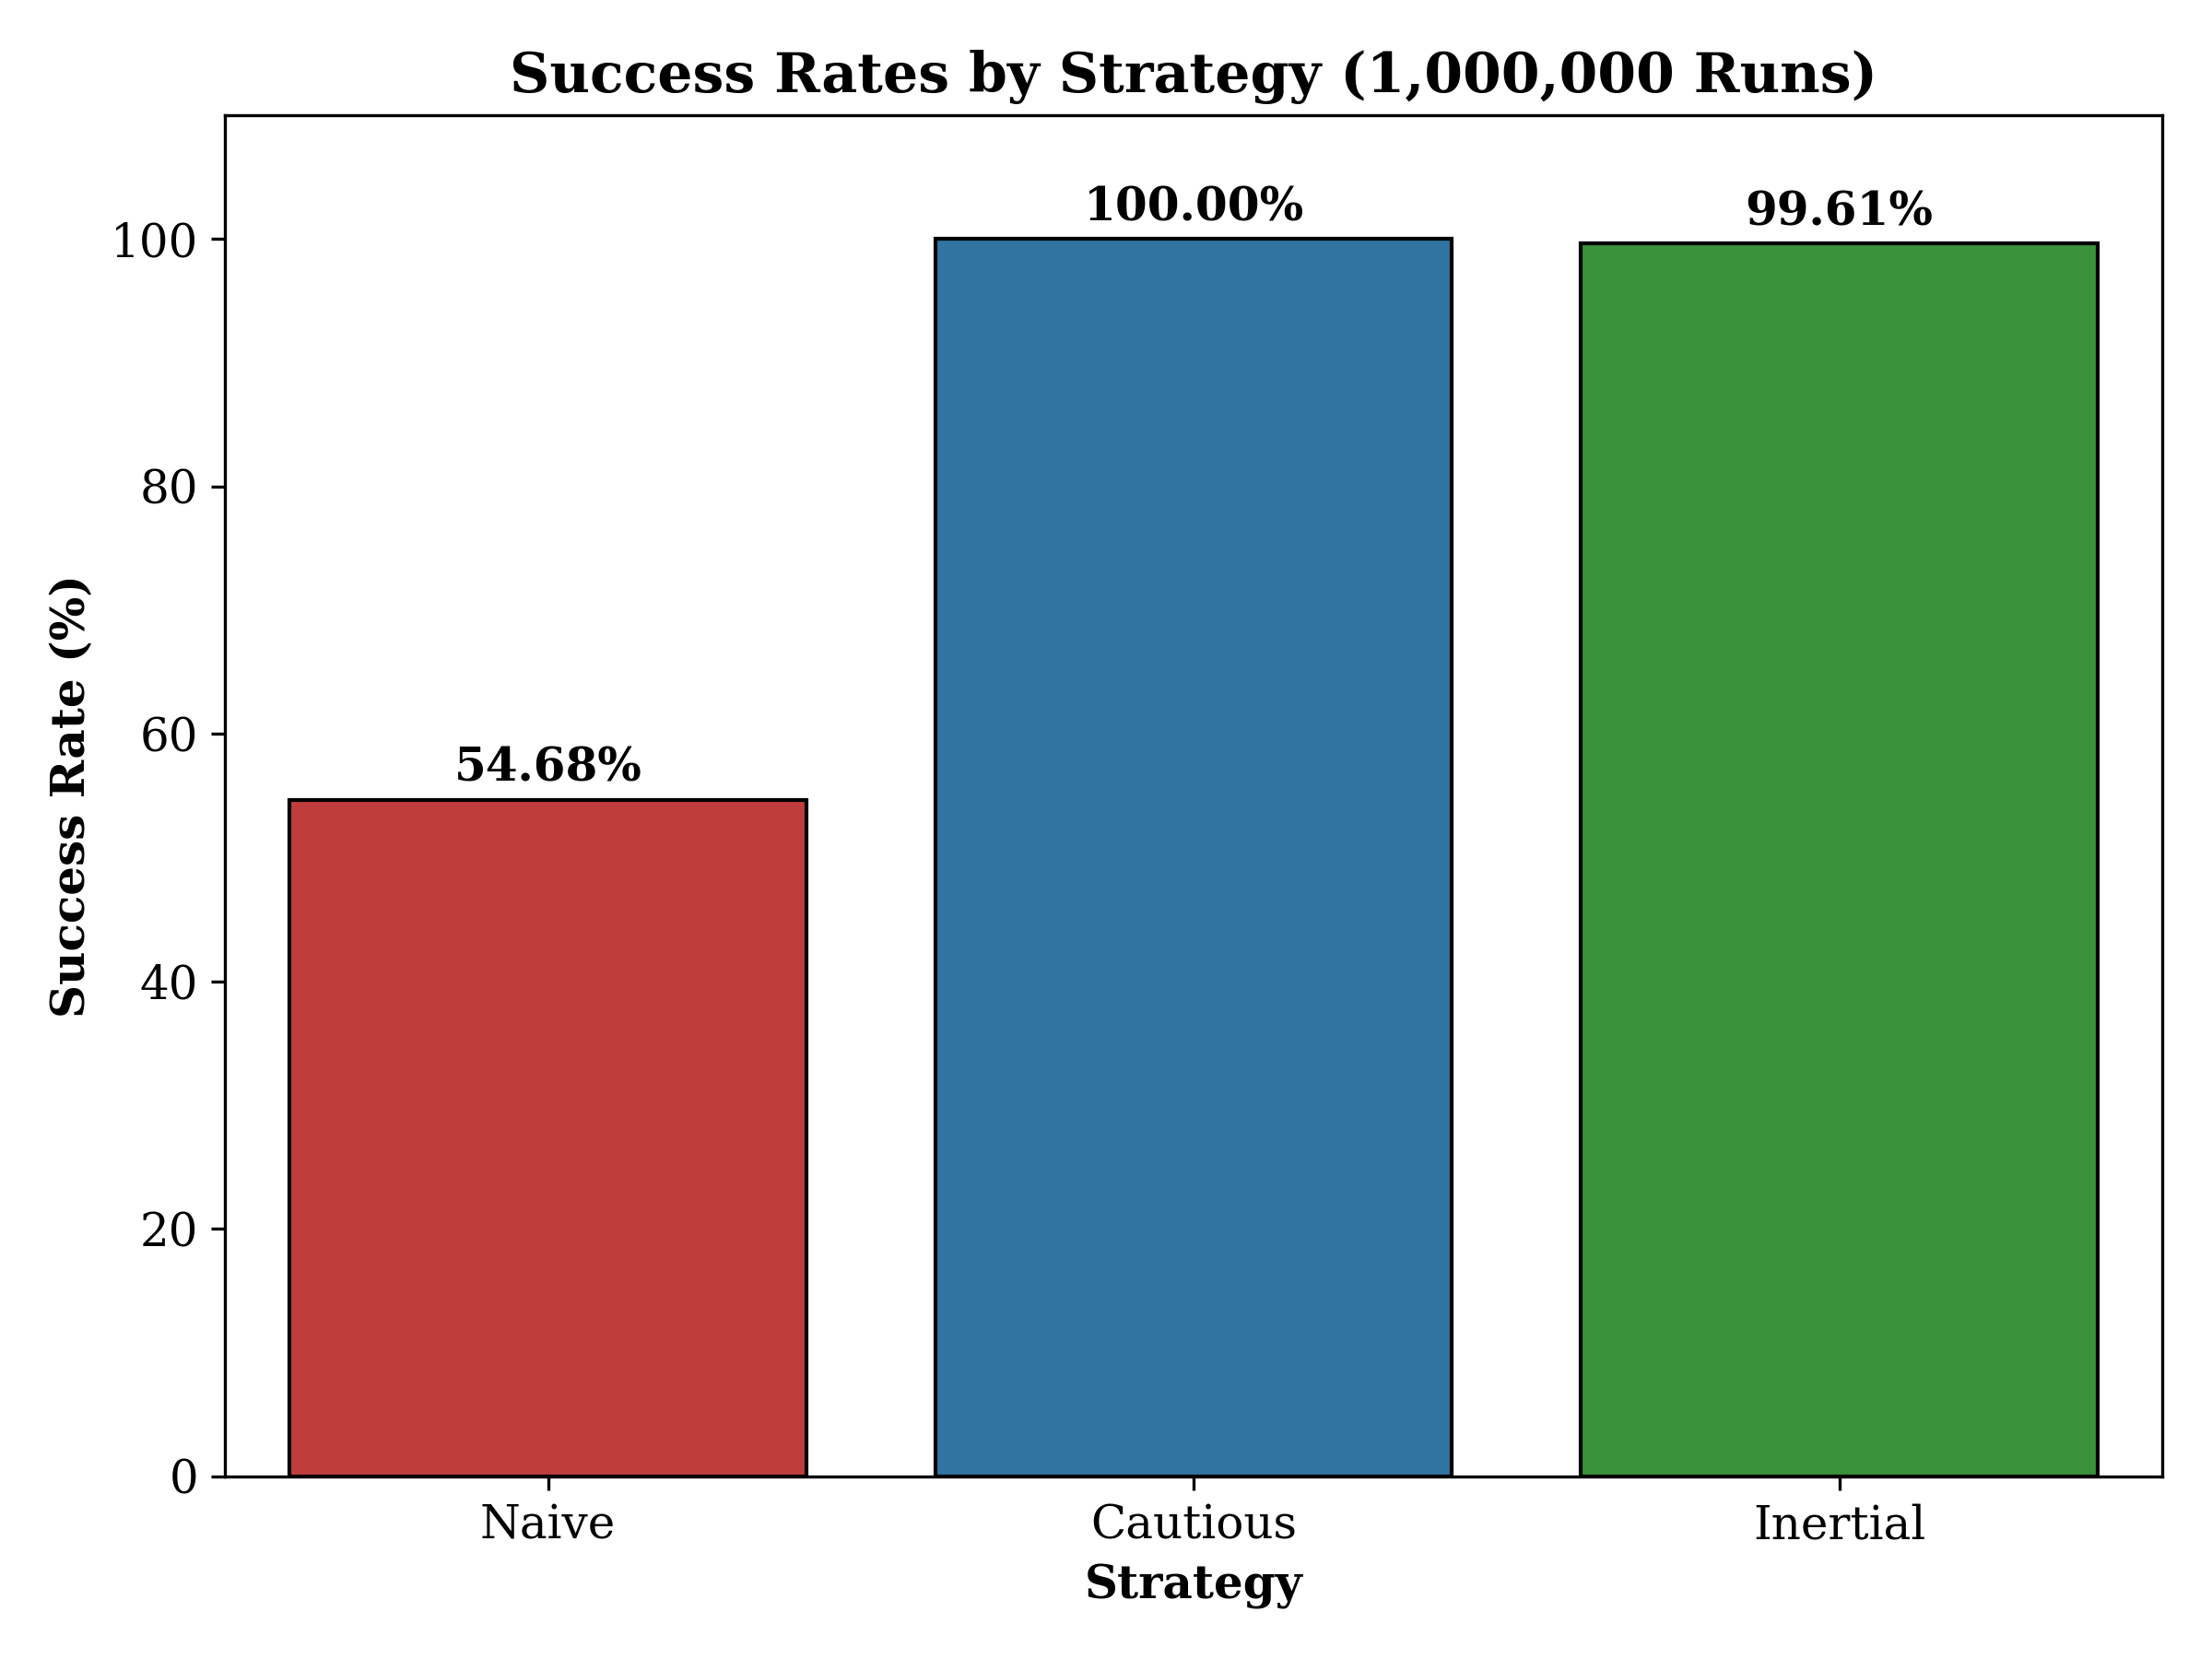
\includegraphics[width=\linewidth]{success_rates.png}
        \caption{שיעורי הצלחה ($10^6$ הרצות).}
        \label{fig:succ}
    \end{minipage}\hfill
    \begin{minipage}[t]{0.48\linewidth}
        \centering
        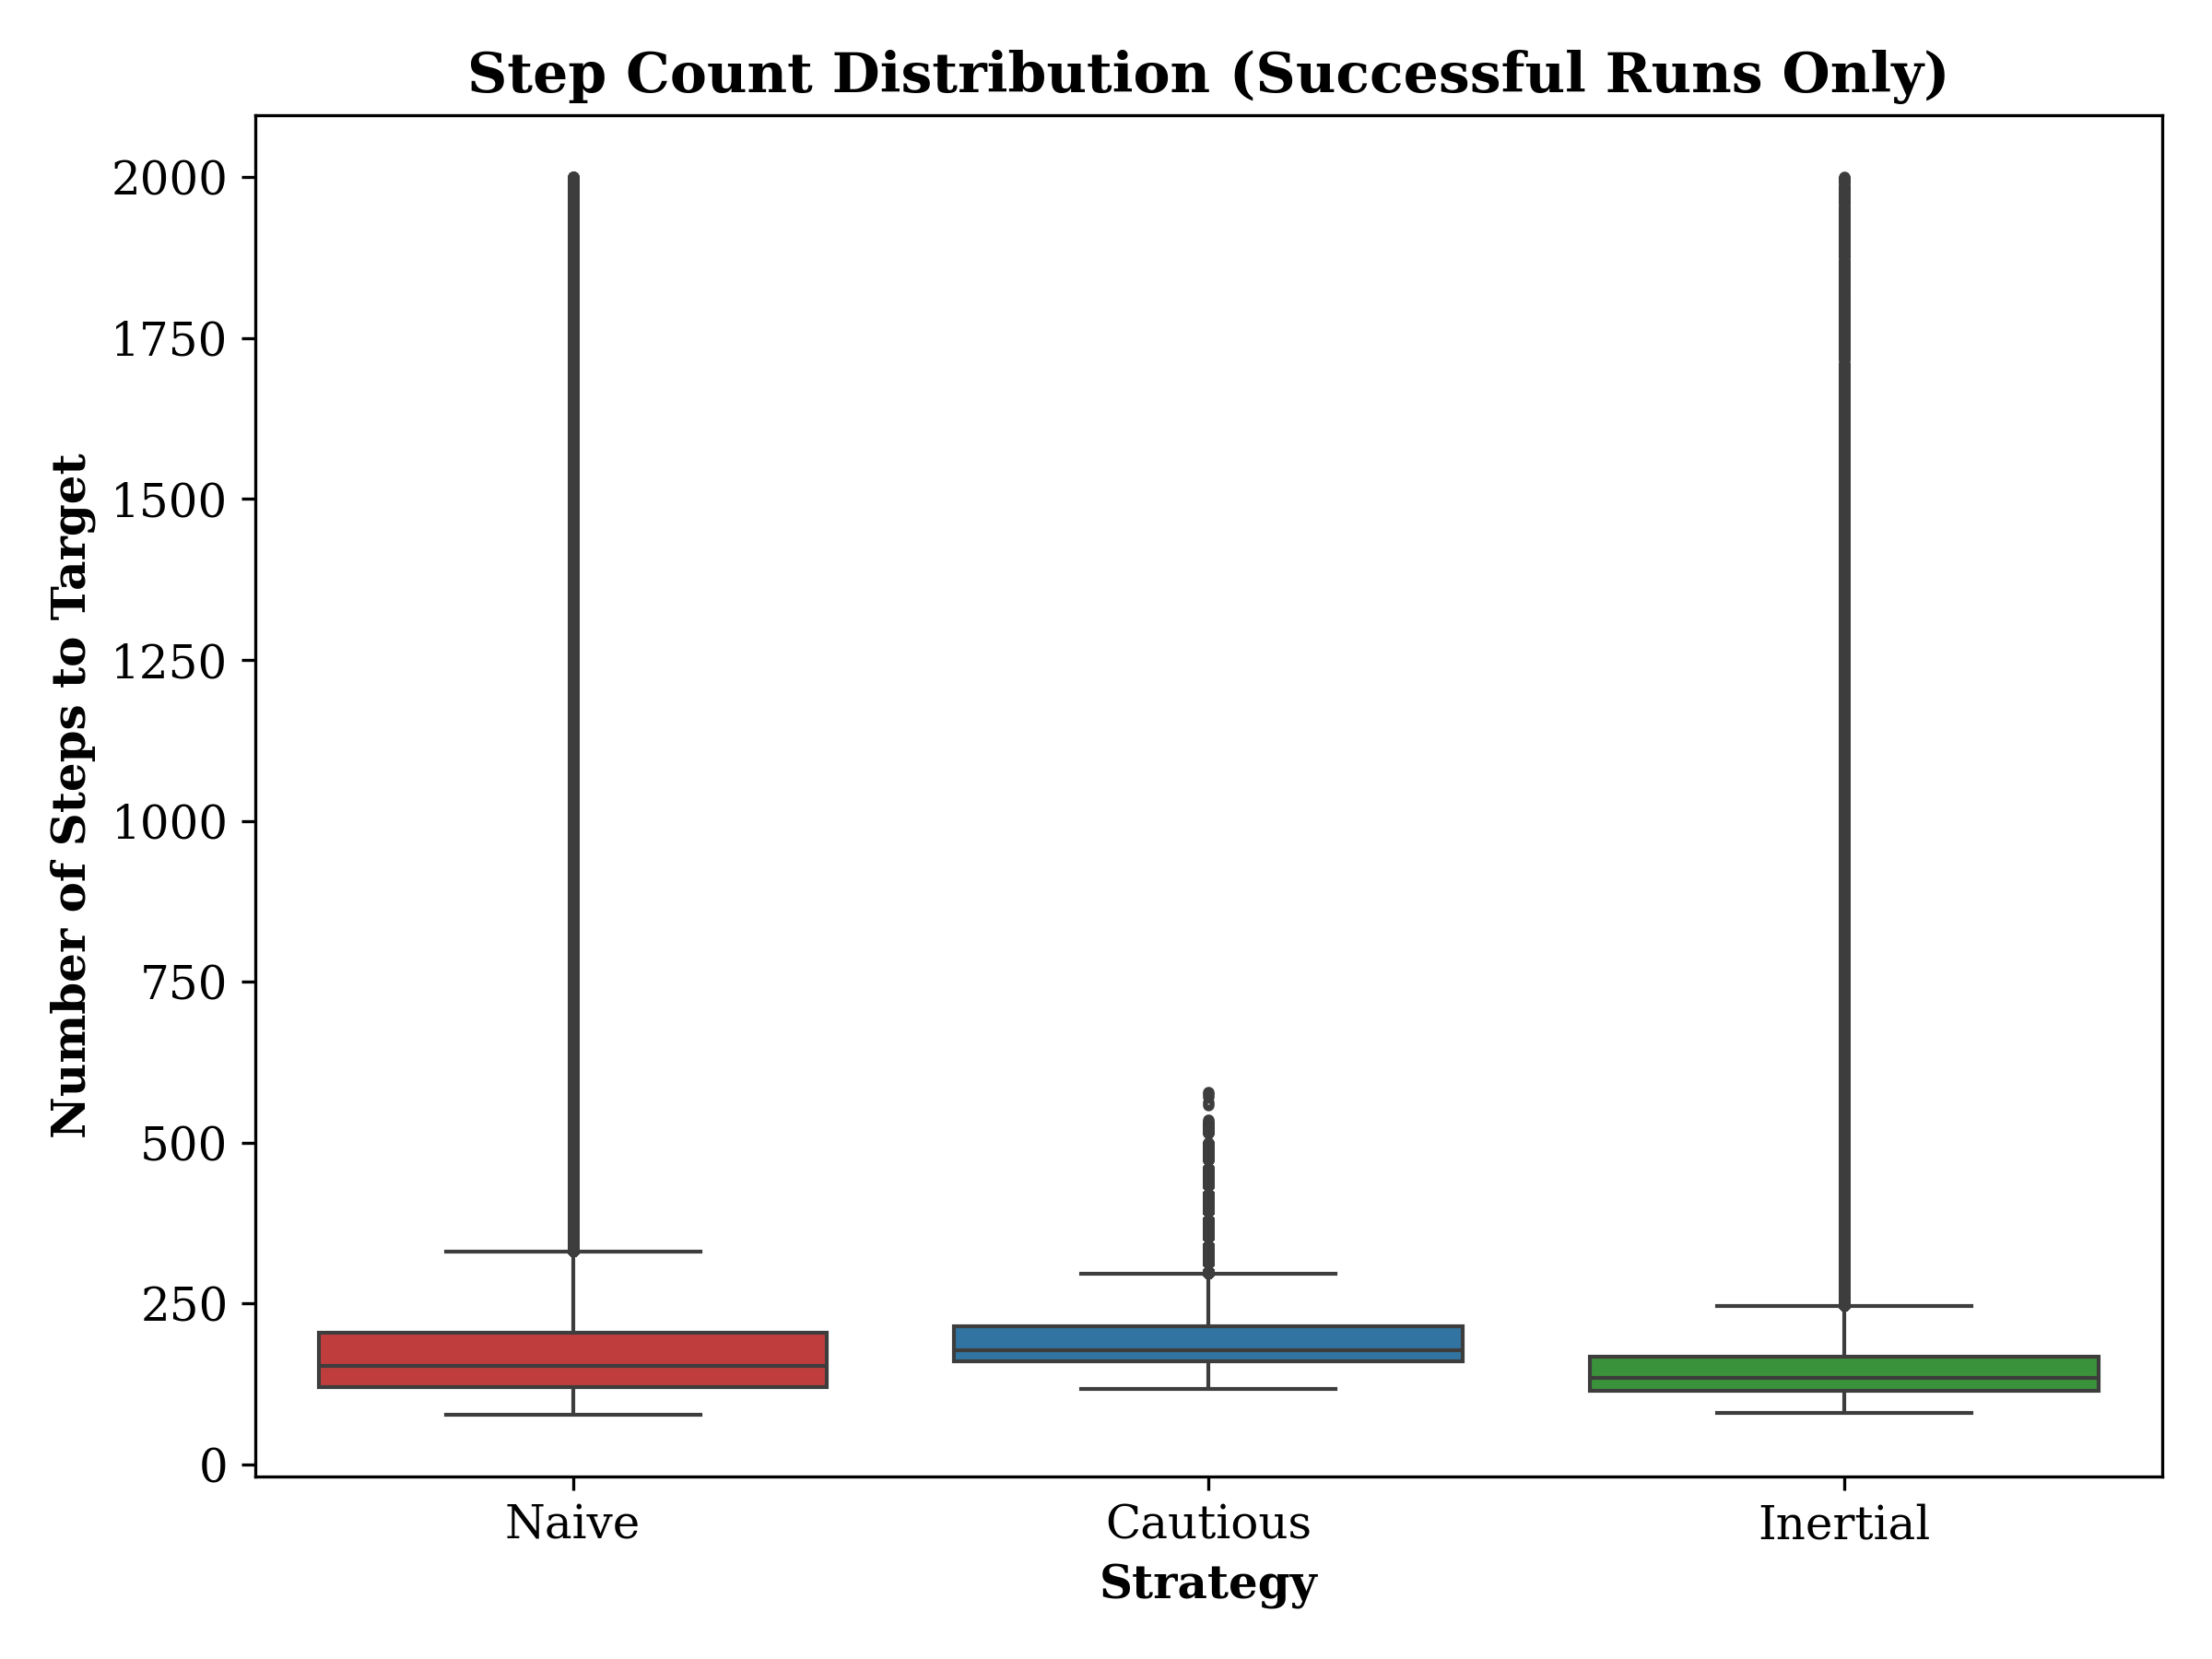
\includegraphics[width=\linewidth]{steps_distribution.png}
        \caption{התפלגות מספר הצעדים.}
        \label{fig:steps}
    \end{minipage}
    \vspace{-1.1em}
\end{figure}

\noindent\textbf{תוצאות ומסקנות.}
טבלה~\ref{tab:results} ואיורים~\ref{fig:succ}–\ref{fig:trap} תומכים בממצאים התאורטיים שלנו תחת התפלגות הסביבות שנדגמה:
(1) אלגוריתם ה-\foreignlanguage{english}{Naive I-Bug} נכשל ב-$45.32\%$ מהסביבות שנדגמו, כאשר כישלונות מייצגים מדגימים הסטת גרדיאנט והרעלת סף (למשל $i_H = 1.230$ באיור~\ref{fig:trap}).
(2) תחת הנחות~\ref{assump:superposition}–\ref{assump:discontinuity}, אסטרטגיית \foreignlanguage{english}{Cautious} משיגה $100.00\%$ הצלחה נצפית ($10^6 / 10^6$ הרצות, זמן סיום מקסימלי נצפה של $578$ צעדים; $137$ צעדים באיור~\ref{fig:trap}), בהתאם למשפט~\ref{thm:cautious}.
(3) בקרב הריצות המוצלחות, ההיוריסטיקה ה-\foreignlanguage{english}{Inertial} מקצרת את ממוצע הצעדים ב-$20.5\%$ ($153.4$ לעומת $193.0$ צעדים; וב-$16.8\%$ במדד הבלתי-מותנה $\bar{N}_{\text{capped}} = 160.6$), תוך כישלון ב-$0.39\%$ ($3,877$) מהניסויים; הכישלונות הנצפים עקביים עם מנגנון נעילת הפאזה של טענה~\ref{prop:resonance}, כפי שמודגם באיור~\ref{fig:trap} ($i_H = 0.167$). תוצאות אלו מבססות שקלול תמורות (\foreignlanguage{english}{Trade-off}) ברור בין בטיחות ליעילות: הקפאת מצב ותנועה מלאה משמרת באופן מותנה את התכנסות \foreignlanguage{english}{I-Bug} התקין תחת מתקפת מדרגה לסירוגין (למעט מתקפות רציפות, משופעות אטית או מתחת לסף), בעוד שהמשך תנועה בחוג פתוח ממקסם מהירות כאשר לכידות תהודה נדירות הן נסבלות או מופחתות באמצעות עירור אקראי.

\begin{figure}[htbp]
    \centering
    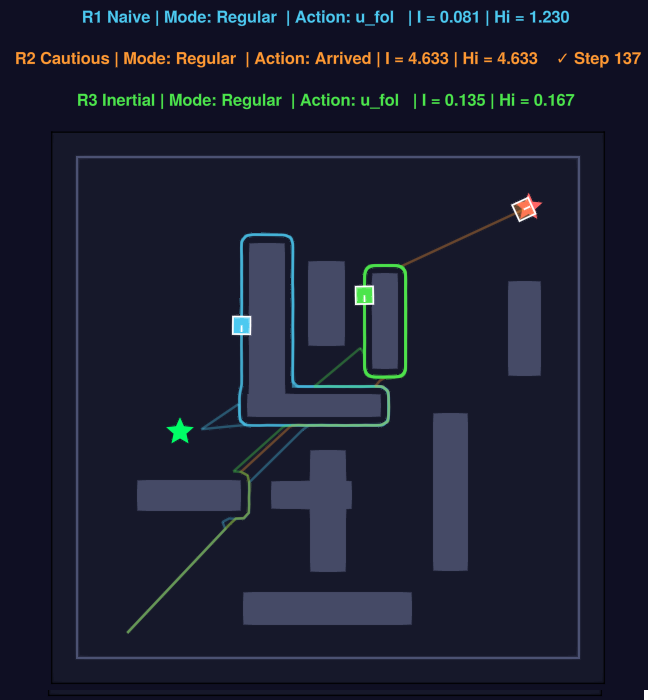
\includegraphics[width=0.68\linewidth]{simulation_trap.png}
    \caption{כישלון כפול מייצג: \foreignlanguage{english}{Naive} (תכלת) מורעל-סף במכשול ה-\foreignlanguage{english}{L}; \foreignlanguage{english}{Inertial} (ירוק) נלכד בלולאת שפה מסונכרנת-פאזה; \foreignlanguage{english}{Cautious} (כתום) ממתין בזמן התקיפה ומגיע למטרה.}
    \label{fig:trap}
    \vspace{-0.8em}
\end{figure}

\begin{otherlanguage}{english}
\begin{thebibliography}{8}
\footnotesize
\setlength{\itemsep}{0pt}
\bibitem{lumelsky1987path}
V.~J. Lumelsky and A.~A. Stepanov, ``Path-planning strategies for a point mobile automaton moving amidst unknown obstacles of arbitrary shape,'' \textit{Algorithmica}, vol.~2, no.~1, pp.~403--430, 1987.

\bibitem{kamon1998tangentbug}
I.~Kamon, E.~Rimon, and E.~Rivlin, ``TangentBug: A range-sensor-based navigation algorithm,'' \textit{Int. J. Robot. Res.}, vol.~17, no.~9, pp.~934--953, 1998.

\bibitem{taylor2009ibug}
K.~Taylor and S.~M. LaValle, ``I-Bug: An intensity-based bug algorithm,'' in \textit{Proc. IEEE Int. Conf. Robot. Autom. (ICRA)}, 2009, pp.~3981--3986.

\bibitem{taylor2014intensity}
K.~Taylor and S.~M. LaValle, ``Intensity-based navigation with global guarantees,'' \textit{Auton. Robots}, vol.~36, no.~4, pp.~349--364, 2014.

\bibitem{kerns2014unmanned}
A.~J. Kerns, D.~P. Shepard, J.~A. Bhatti, and T.~E. Humphreys, ``Unmanned aircraft capture and control via GPS spoofing,'' \textit{J. Field Robot.}, vol.~31, no.~4, pp.~617--636, 2014.

\bibitem{psiaki2016gnss}
M.~L. Psiaki and T.~E. Humphreys, ``GNSS spoofing and detection,'' \textit{Proc. IEEE}, vol.~104, no.~6, pp.~1258--1270, 2016.

\bibitem{giraldo2018survey}
J.~Giraldo \textit{et al.}, ``A survey of physics-based attack detection in cyber-physical systems,'' \textit{ACM Comput. Surv.}, vol.~51, no.~4, Art.~no.~76, pp.~1--36, 2018.

\bibitem{basseville1993detection}
M.~Basseville and I.~V. Nikiforov, \textit{Detection of Abrupt Changes: Theory and Application}. Englewood Cliffs, NJ, USA: Prentice Hall, 1993.
\end{thebibliography}
\end{otherlanguage}

\end{document}
